\vspace{\baselineskip}

\hspace{0,5cm}Notre expérience s'est divisée en deux axes. Le premier axe
consiste à déterminer comprendre et étudier le style d'écriture de Molière et de
Corneille. Le second axe consiste à déterminer les clusters de textes qui se
ressemblent le plus.

\hspace{0,5cm}Grâce à la bibliothèque \textbf{NLTK} et \textbf{WorldCloud}, nous
avons pu faire un nuage de mot pour le corpus de Molière. Un nuage de mots est
une manière de visualiser la fréquence des mots dans un corpus. Les mots les
plus fréquents sont présentés sous forme de nuage, où la taille du mot est
proportionnelle à sa fréquence. Cette représentation peut donner une vue
d'ensemble rapide des termes les plus courants dans le corpus de Molière. Pour
que l'analyse soit plus pertinente nous avons supprimé la prise en compte des
noms propres, qui sont uniques aux oeuvres.

\begin{figure}[htbp]
    \centering
    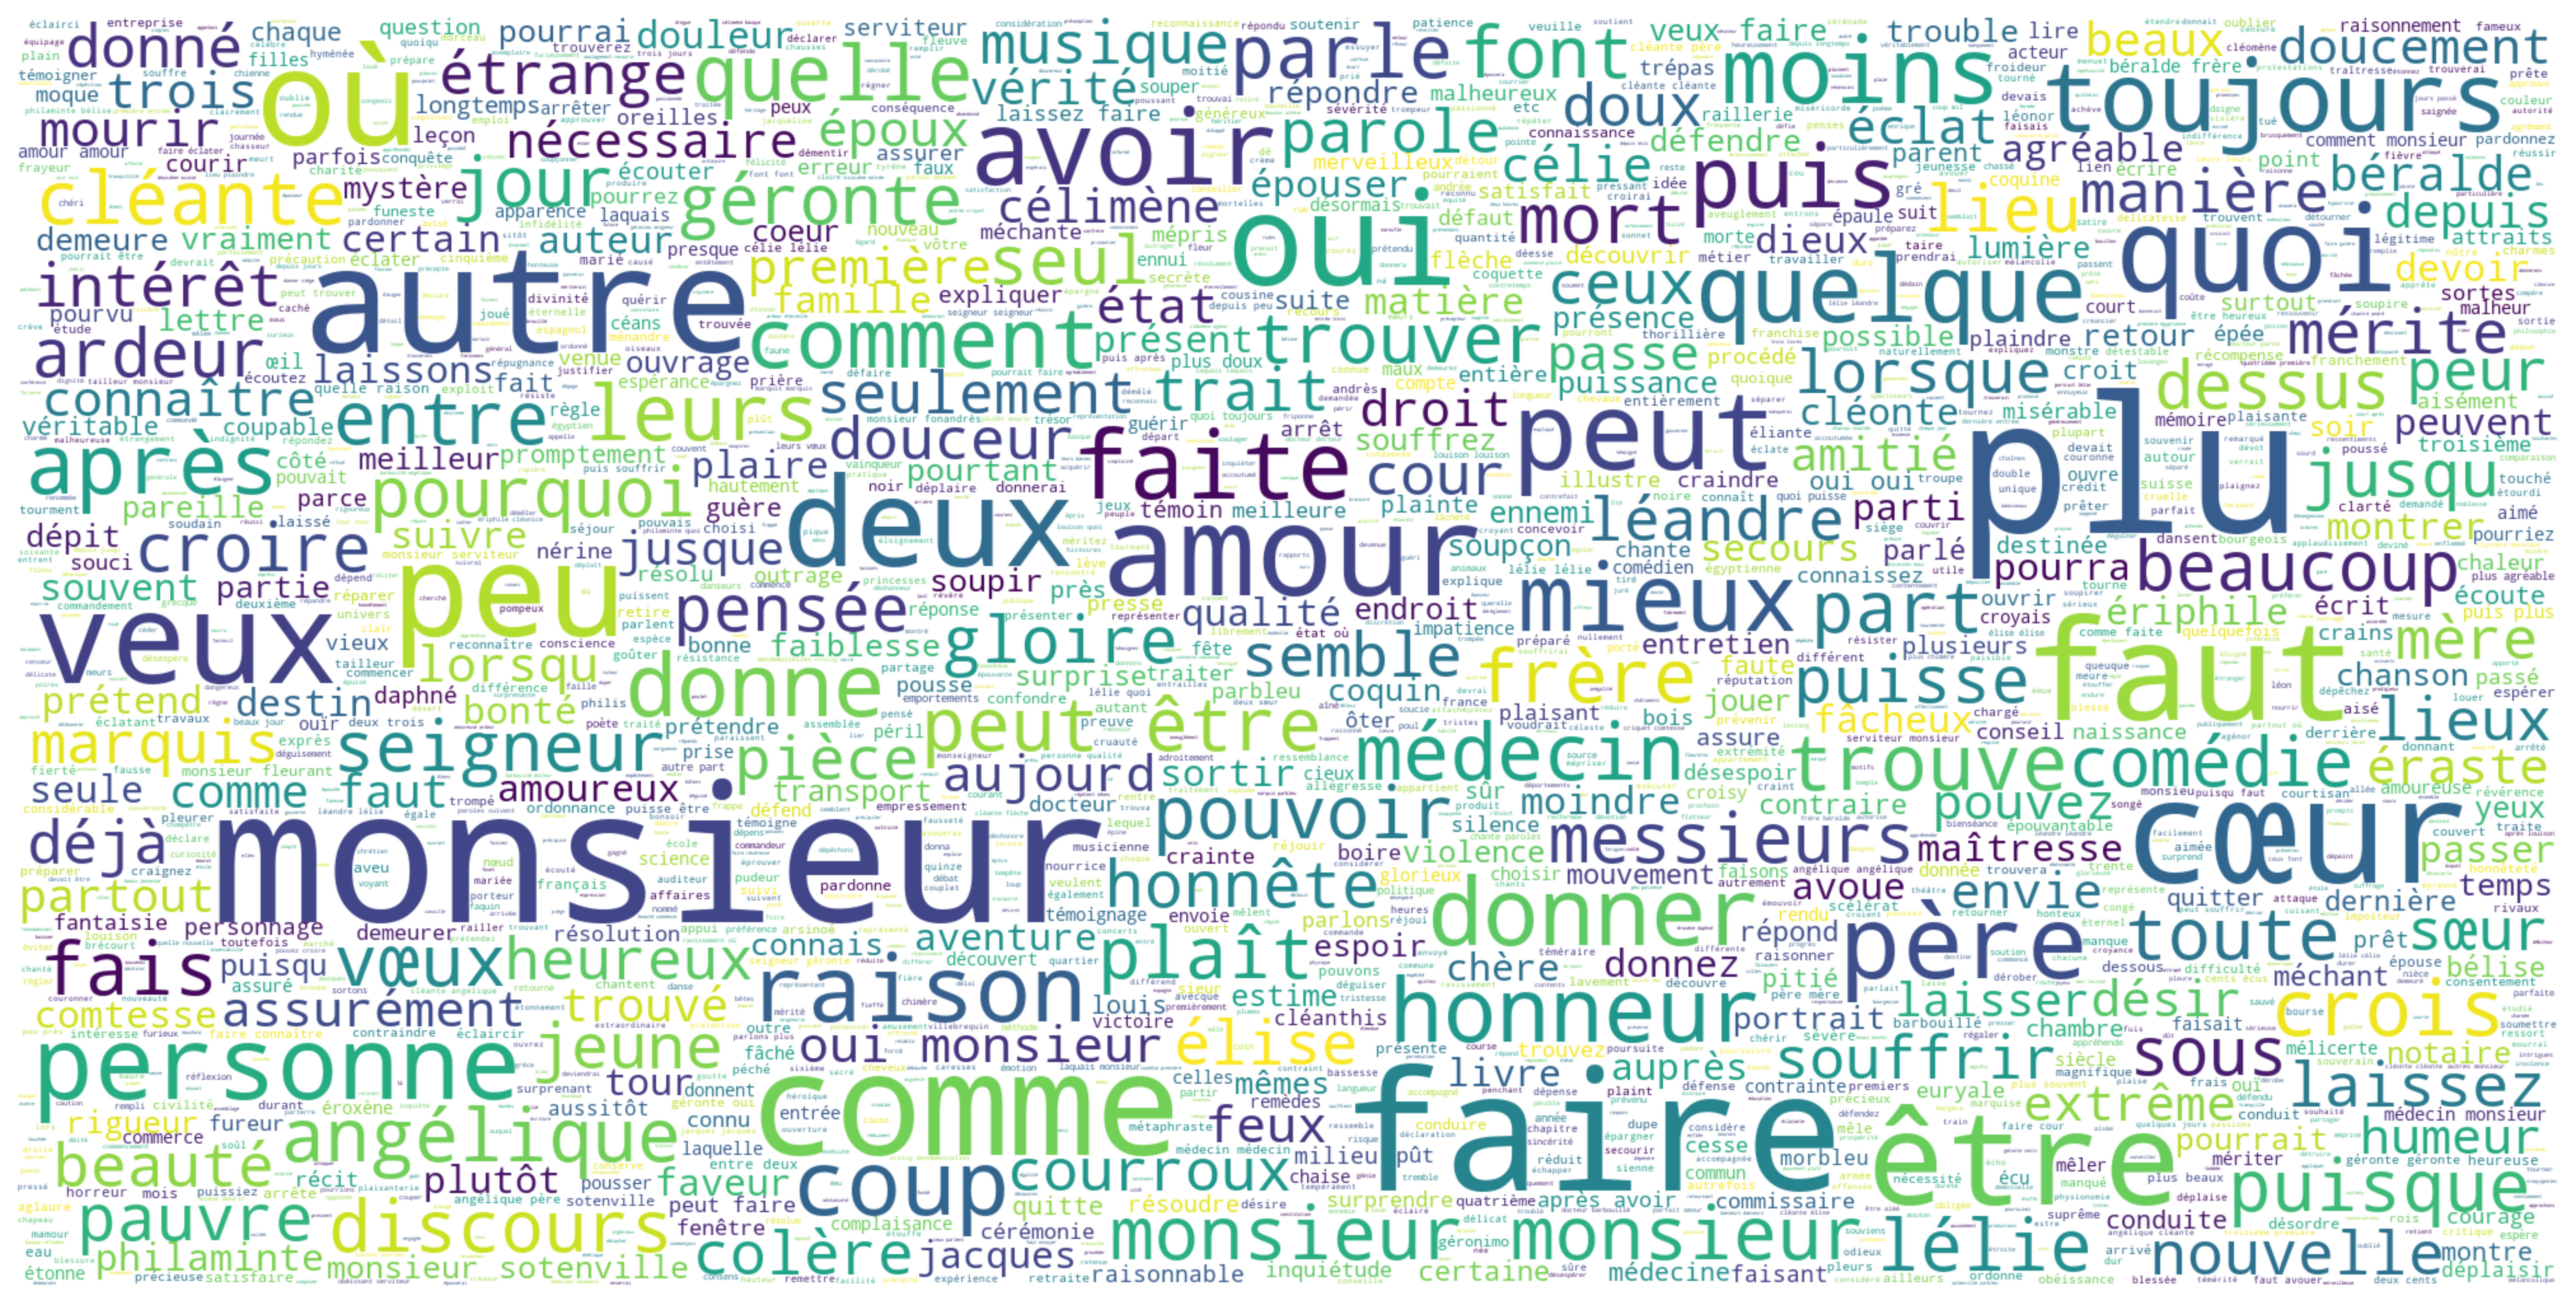
\includegraphics[width=15cm]{Ressources/nuage_sans_noms.png}
    \caption{Nuage de mots du corpus de Molière}
    \label{fig:images}
  \end{figure}

\vspace{\baselineskip}
\newpage
\hspace{0,5cm}Grâce au nuage de mots, nous avions remarqué que le mot
\textit{Monsieur} revenait très souvent. Cette grande importance du mot
\textit{Monsieur} dans le nuage de mots révèle le vocabulaire et les règles
d'écriture de l'époque.  \\Afin de mieux comprendre le style d'écriture de
Molière, nous avons également réaliser un histograme des mots les plus fréquents
dans le corpus de Molière.  Pour rendre ce diagramme plus pertinent, nous avons
décidé de ne pas prendre en compte les noms de personnages et le mot
\textit{Monsieur}.

\begin{figure}[htbp]
    \centering
    \includegraphics[width=13cm]{Ressources/diagr_sans_noms_mosn.png}
\caption{Diagramme de mots du corpus de Molière sans le mot \textit{Monsieur}}
    \label{fig:images}
  \end{figure}

  \vspace{\baselineskip}

\hspace{0,5cm}En répétant l'éxpérience sur le corpus de Corneille, nous trouvons
des résultats assez similaires.

\begin{figure}[htbp]
  \centering
  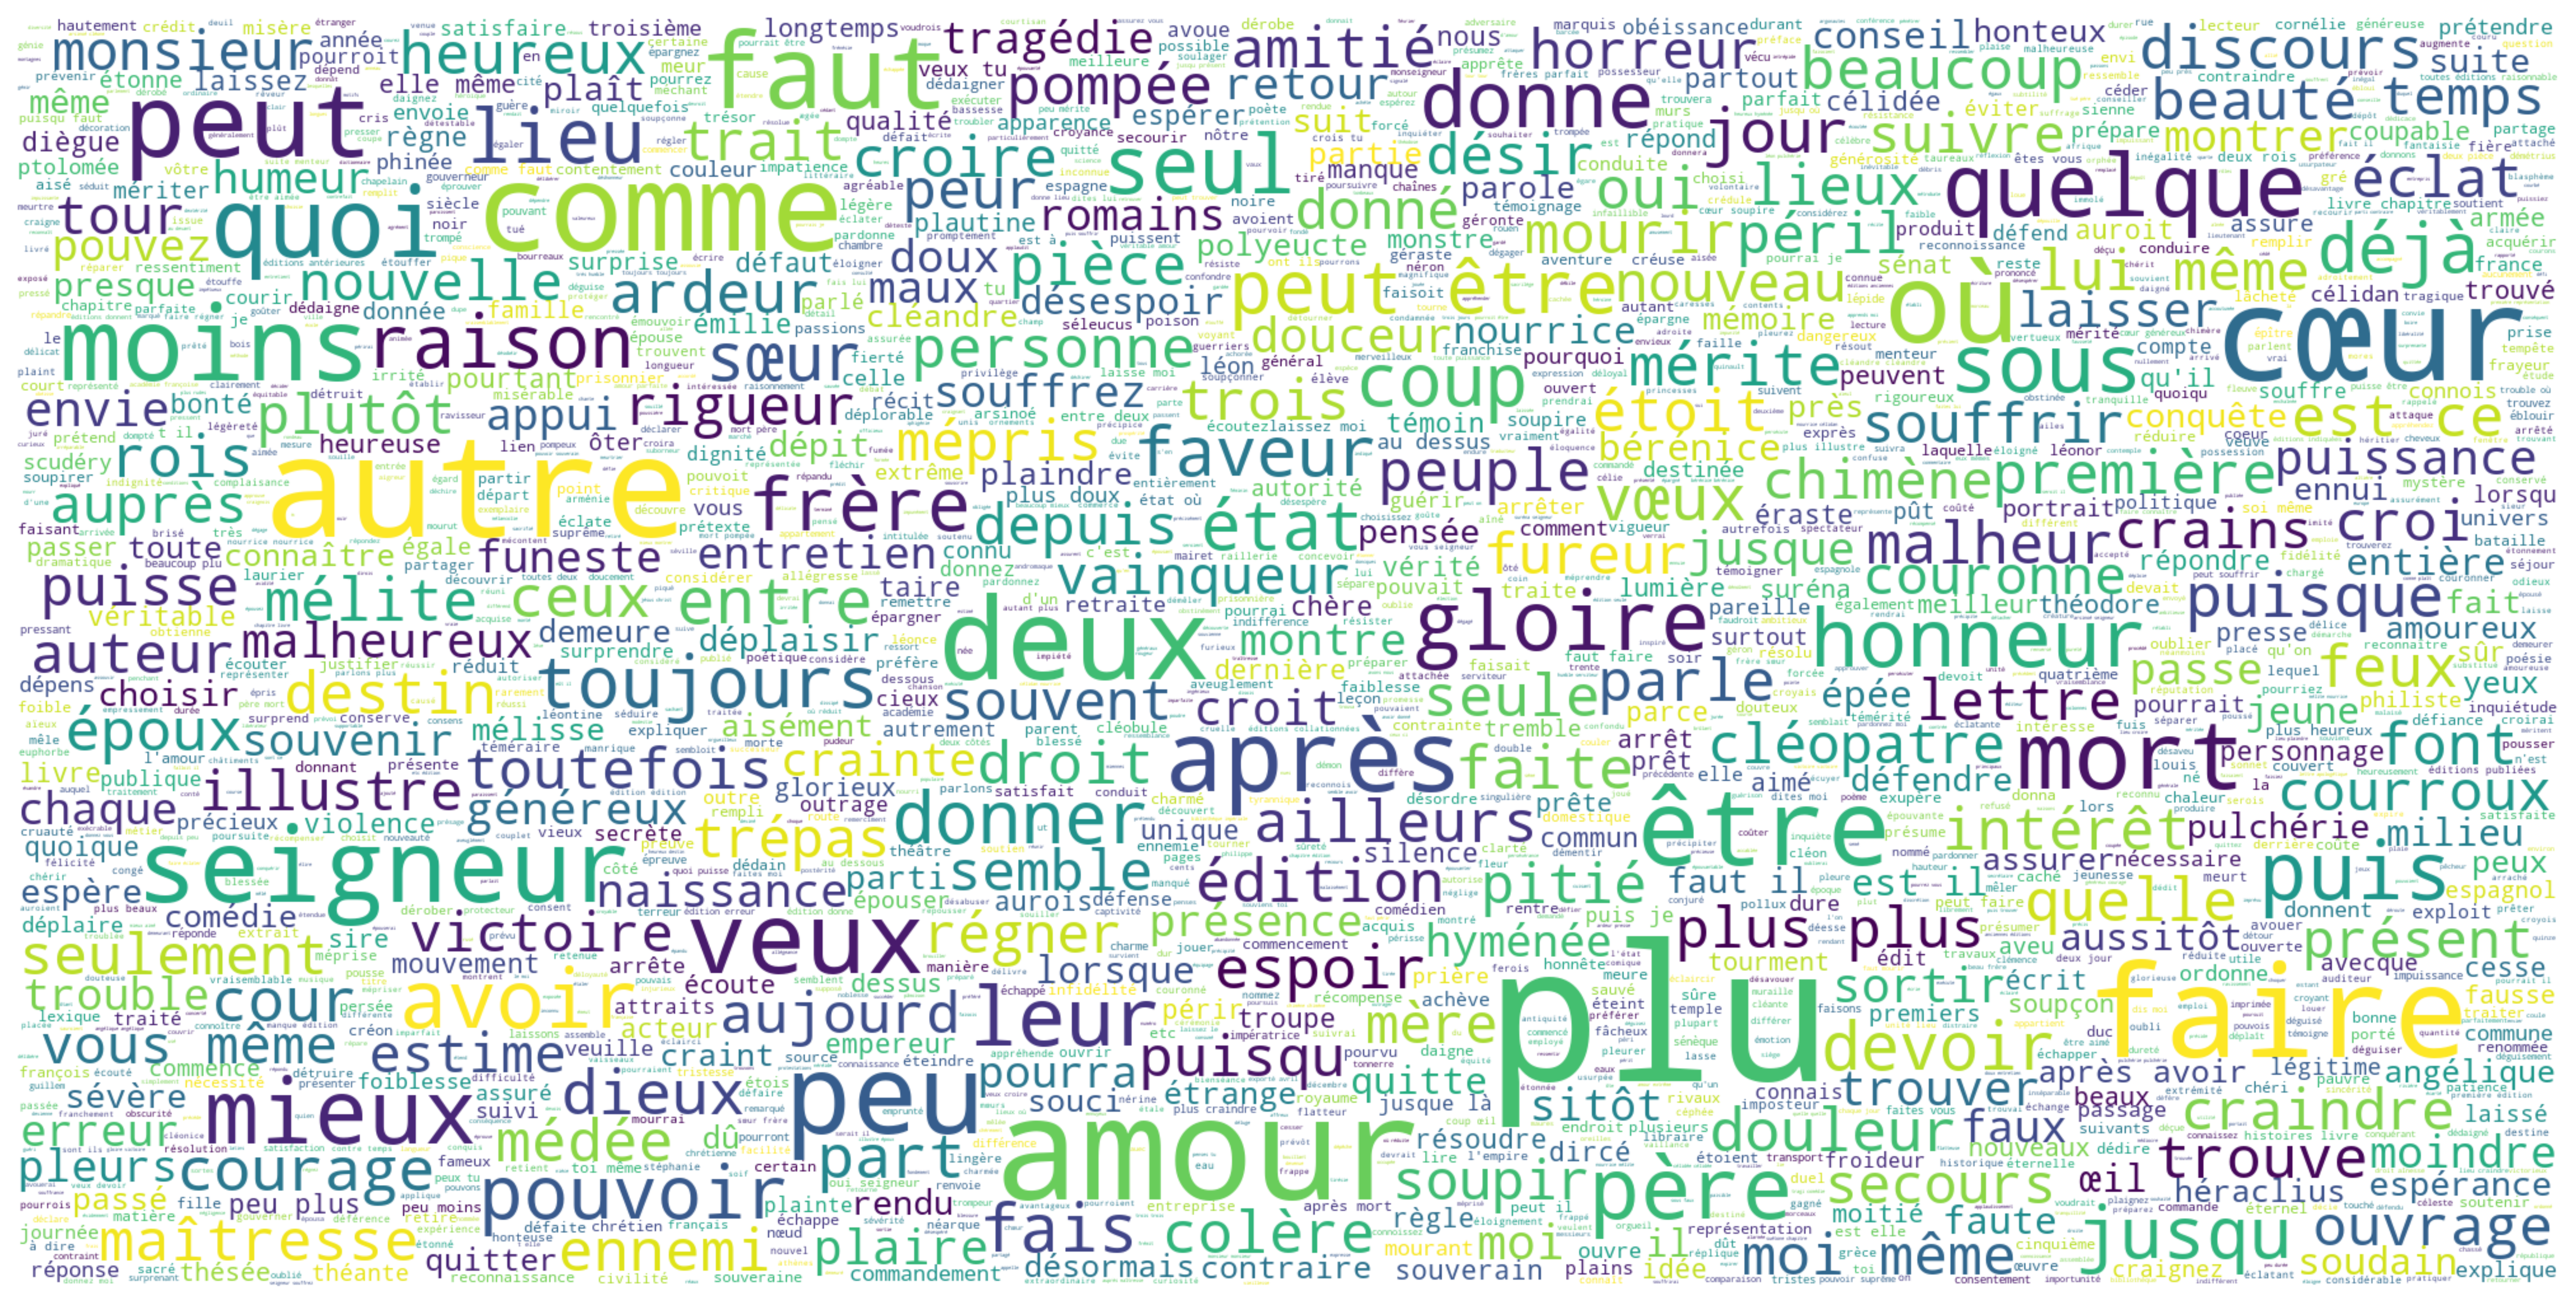
\includegraphics[width=15cm]{Ressources/nuage_de_mots-Corneille.png}
  \caption{Nuage de mots du corpus de Corneille}
  \label{fig:images}
\end{figure}

\begin{figure}[htbp]
  \centering
  \includegraphics[width=18cm]{Ressources/corneille_digramme.png}
  \caption{Diagramme de mots du corpus de Corneille}
  \label{fig:images}
\end{figure}

\newpage

\hspace{0,5cm}Grâce à l'analyse des nuages de mots, nous constatons une utilisation
quasi similaire du mot \textit{plu}, \textit{amour} ou encore \textit{cœur} .
Ces utilisations fréquentes des mots par nos deux auteurs peut rendre difficile
l'attribution précise de l'auteur d'une œuvre en se basant uniquement sur la
distance euclidienne inter-textuelle, comme celle proposée par D. et C. Labbé.
Cela souligne l'importance d'utiliser des métriques et des méthodes d'analyse
supplémentaires pour une identification plus précise de l'auteur.

\vspace{\baselineskip}

\hspace{0,5cm}Nous avons ensuite réalisé une analyse de bigrammes et trigrammes. En analysant
les paires de mots (bigrammes) ou les groupes de trois mots (trigrammes) qui se
produisent souvent ensemble dans les textes de Molière et de Corneille, nous
avons pu comprendre davantage sur les expressions idiomatiques, les tournures de
phrases et les habitudes stylistiques distinctes des auteurs.
\\Les résultats se présentent sous la forme d'un fichier texte répertoriant tous
les bigrammes différents fréquemment associés ainsi que les groupes de
trigrammes qui apparaissent ensemble avec leur fréquence respective.
	
\hspace{0,5cm}Nous avons constaté que le digramme (peut, être) est plus fréquent,
avec 235 occurrences, dans les œuvres de Molière, tandis que chez Corneille,
c'est le digramme (après, avoir) qui revient le plus souvent, avec 117
occurrences. Nous remarquons aussi peu de différences entre les frequences de
certains digrammes similaires, comme (puis, plus) qui se répète 44 fois chez
Corneille et 33 fois chez Molière.
\\Au niveau des trigrammes, le triplet de mots le plus fréquent chez Molière est
(monsieur, oui, monsieur), tandis que chez Corneille, c'est (plus, puis, faire).
Nous ne remarquons pas de trigrammes similaires, en revanche le champs lexical
est très proche, avec des mots comme monsieur, oui, puis, plus qui reviennent
souvent.

\vspace{\baselineskip}

\hspace{0,5cm}Notre second axe d'analyse consiste à déterminer les clusters de
textes qui se ressemblent le plus. Après avoir réalisé un prétraitement (où nous
reviendrons en détails dans la partie 3.4) de compléxité globale O(n\(^2)\), et
avoir vectoriser nos textes, nous avons pu réaliser des dendrogrammes.
Nous avons appliqué nos algorithmes de clustering, qui comprennent le
k-means utilisant la distance euclidienne et la métrique du cosinus, ainsi que
l'agglomerative Clustering utilisant la distance de Jaccard. Les mesures
d'agrégation des clusters que nous avons utilisées sont "complete" et
"average". En ce qui concerne la complexité de nos algorithmes, elle dépend de
plusieurs facteurs tels que la taille des données et le nombre de clusters.

\begin{figure}[htbp]
  \centering
  \includegraphics[width=15cm]{Ressources/Dendo_eucli.png}
  \caption{Dendrogramme suivant la distance euclidienne}
  \label{fig:images}
\end{figure}

\newpage
\begin{figure}[htbp]
  \centering
  \includegraphics[width=15cm]{Ressources/Dendo_cos.png}
  \caption{Dendrogramme suivant la distance cosinus}
  \label{fig:images}
\end{figure}

\newpage
\begin{figure}[htbp]
  \centering
  \includegraphics[width=15cm]{Ressources/Dendo_Jacard.png}
  \caption{Dendrogramme suivant la similarité de Jaccard}
  \label{fig:images}
\end{figure}

\newpage

\hspace{0,5cm}Lors de l'interprétation des résultats sur les dendrogrammes, nous constatons
que certaines œuvres ne sont pas bien positionnées lorsque nous utilisons la
distance euclidienne et la métrique du cosinus. En revanche, avec la métrique de
Jaccard, nous observons des regroupements plus compacts, que ce soit pour les
œuvres de Molière ou de Corneille. Cela suggère que la métrique de Jaccard est
plus efficace pour capturer les similitudes et les différences entre les textes,
grâce a son approche ensembliste qui le différencie des autres métriques. 
Ce qu'appuie notre étude, en considérons que
l'approche et les choix des caractéristiques et des métriques sont plus pertinents
dans la méthodologie développée par Mr Caffiero et Mr Camps, est qu'une étude
stylométrique sur des textes littéraires si proches nécessite une approche plus
fine et plus précise. La diffculté de l'attribution de l'auteur est d'autant
plus grande que les auteurs sont proches stylistiquement.